\documentclass{article}

\usepackage{amsmath}
\usepackage{graphicx}
\usepackage{float}
\usepackage{pdflscape}
\usepackage{natbib}
\usepackage[margin=1in]{geometry}
\usepackage[document]{ragged2e}
\setlength{\parindent}{4em}

\author{Stephen M. Lee}
\title{Variation in Political News \\ \large{An NLP Approach}}

\begin{document}
	%%%%%%%%%%%%%%%%%%%%%%%%%%%%%%%%%%%%%%%%%%%%%%%%
	% HOUSEKEEPING
	
	\maketitle 
	
	\newpage
	
	\abstract{By many reports, there has been an increase in skepticism and polarity in news consumption. Since 2016, we have even heard the president of the United States make accusations of mainstream news sources publishing ``fake news''. With a goal of classifying articles by their news source, I scraped several thousand political news articles from Fox, Vox, and PBS News. I then train a bidirectional LSTM netural network to classify the source of the article based on the text and find that it can accurately predict the correct source. Finally, I develop a simple web application that utilizes the trained network and discuss the social implications of such a tool.}
		
	\newpage
	
	\tableofcontents
	
	\newpage
	
	%%%%%%%%%%%%%%%%%%%%%%%%%%%%%%%%%%%%%%%%%%%%%%%%
	% INTRO
	
	\vspace{2\baselineskip}
	\begin{center}
		\textit{``If you can't measure it, you can't improve it.''}
	\end{center}
	\begin{flushright}
		--- Peter Drucker
	\end{flushright}

	\vspace{2\baselineskip}
	
	\section{Introduction}
	
		The 2016 United States Presidential Election, to many, raised questions as to the reliability of their news sources. For example, \citet{allcott2017social} estimate that the average US adult read and remembered about one, and possibly up to several, fake news articles during the election period. While they make no statements about the effects of this exposure, the implications are certainly thought provoking. 
		
		Since then, many social media companies and other institutions have begun public campaigns to combat the perceived threat from fake news, including explicit efforts from Google and Facebook to remove ``fake news sites'', as documented in \citet{allcott2017social}. 
		
		With a goal of classifying articles by their news source, I scraped several thousand news articles from Fox, Vox, and PBS News. By some estimations,\footnote{The website https://www.adfontesmedia.com/ provides a visual representation of media bias. Their methodology is well documented, and the outcome is largely consistent with other sources and anecdotal descriptions of bias.} these three news sites represent distinct categories of news: Fox as a conservative “right” opinion; Vox as a liberal “left” opinion; and PBS as the “center” primary source news position. Figure \ref{fig:news-bias} shows a graphic representation of this news bias. 
		
		I first calculate the top words, 2-gram, and 3-gram frequencies to better understand the dataset, and then train a bidirectional, long-term short-term memory (LSTM) recurrent neural network using the GloVe pretrained word embeddings to predict the source of news. 
		
		In this case, I find that a relatively simple, bidirectional, LSTM recurrent neural network can in fact correctly predict the source of an article with very high accuracy. I then use the result of this trained network to build a web app that can allow for a copy-and-paste interface to this classification model. Depending on the extent to which the underlying model enables transfer learning, this web app could ideally serve as a first check on the inherent bias in political news before you read. 
		
		\subsection{Literature Review}
		
		This work fits into existing literature by bridging gaps between the cutting edge of computer science and economics. On the computer science front, bidirectional LSTM recurrent neural networks provide some of the most accurate results for predicting sequential data. The LSTM architecture was introduced in \citet{hochreiter1997long}, extending the Recurrant Neural Network (RNN) to improve lagged information storage for the purpose of predicting sequential data. More recently, \citet{gers2000recurrent}, \citet{chung2014empirical}, and \citet{yao2015depth} introduce variations on the baseline \citet{hochreiter1997long} LSTM model, although \citet{greff2016lstm} show them all to be roughly equivalent on a variety of prediction tasks. 
		
		\citet{schuster1997bidirectional} introduced the first bidirectional RNN reporting a significant predictive improvements over traditional RNNs. Together, bidirectional LSTM architectures prove to be among the most accurate models for language tasks, consistent with \citet{wang2015unified}. 
		
		The economic work on media bias focuses more on inference based analyses. In particular, \citet{gentzkow2010drives} find that readers prefer to consume ``like-minded'' news---meaning they want to have their prior beliefs validated---and that the profit maximizing response from news companies can account for around 20\% of the variation in political slant or bias. In this same direction, \citet{gentzkow2006media} also find that a theoretical Bayesian consumer will effectively reinforce their beliefs of a given news source quality when they read something that confirms their priors. Together, these works suggest that political news bias may be a tactical response of competing news firms to segment the consumer market according to their heterogeneous beliefs, and, further, that this polarization may be self-reinforcing. In fact, \citet{gentzkow2008competition} go as far as to suggest that competition in information markets may actually be counterproductive in achieving balanced and unbiased news. These effects could explain the relative neutrality of news sources like the BBC that are somewhat insulated from the competitive pressures faced by Fox and Vox news companies. 
		
		If these news companies are in fact biased by construction, can we train a computer to detect and classify the differences based on the language alone? Regardless of the answer, there are substantial implications. If yes, then we can create computer software to help classify news based on language content. This would enable news consumers to effectively ``locate'' their news consumption in the same way that a GPS helps to locate yourself on a map, or a calorie tracking app helps to locate your dietary health. However, if the answer is no, then it provides a clear direction for further study in the field of natural language processing and machine learning insofar as additional context is needed to parse the perceived differences. To my knowledge, this paper provides the first thorough NLP based approach to understanding semantic differences across news sources. 
		
		\begin{figure}[H]
			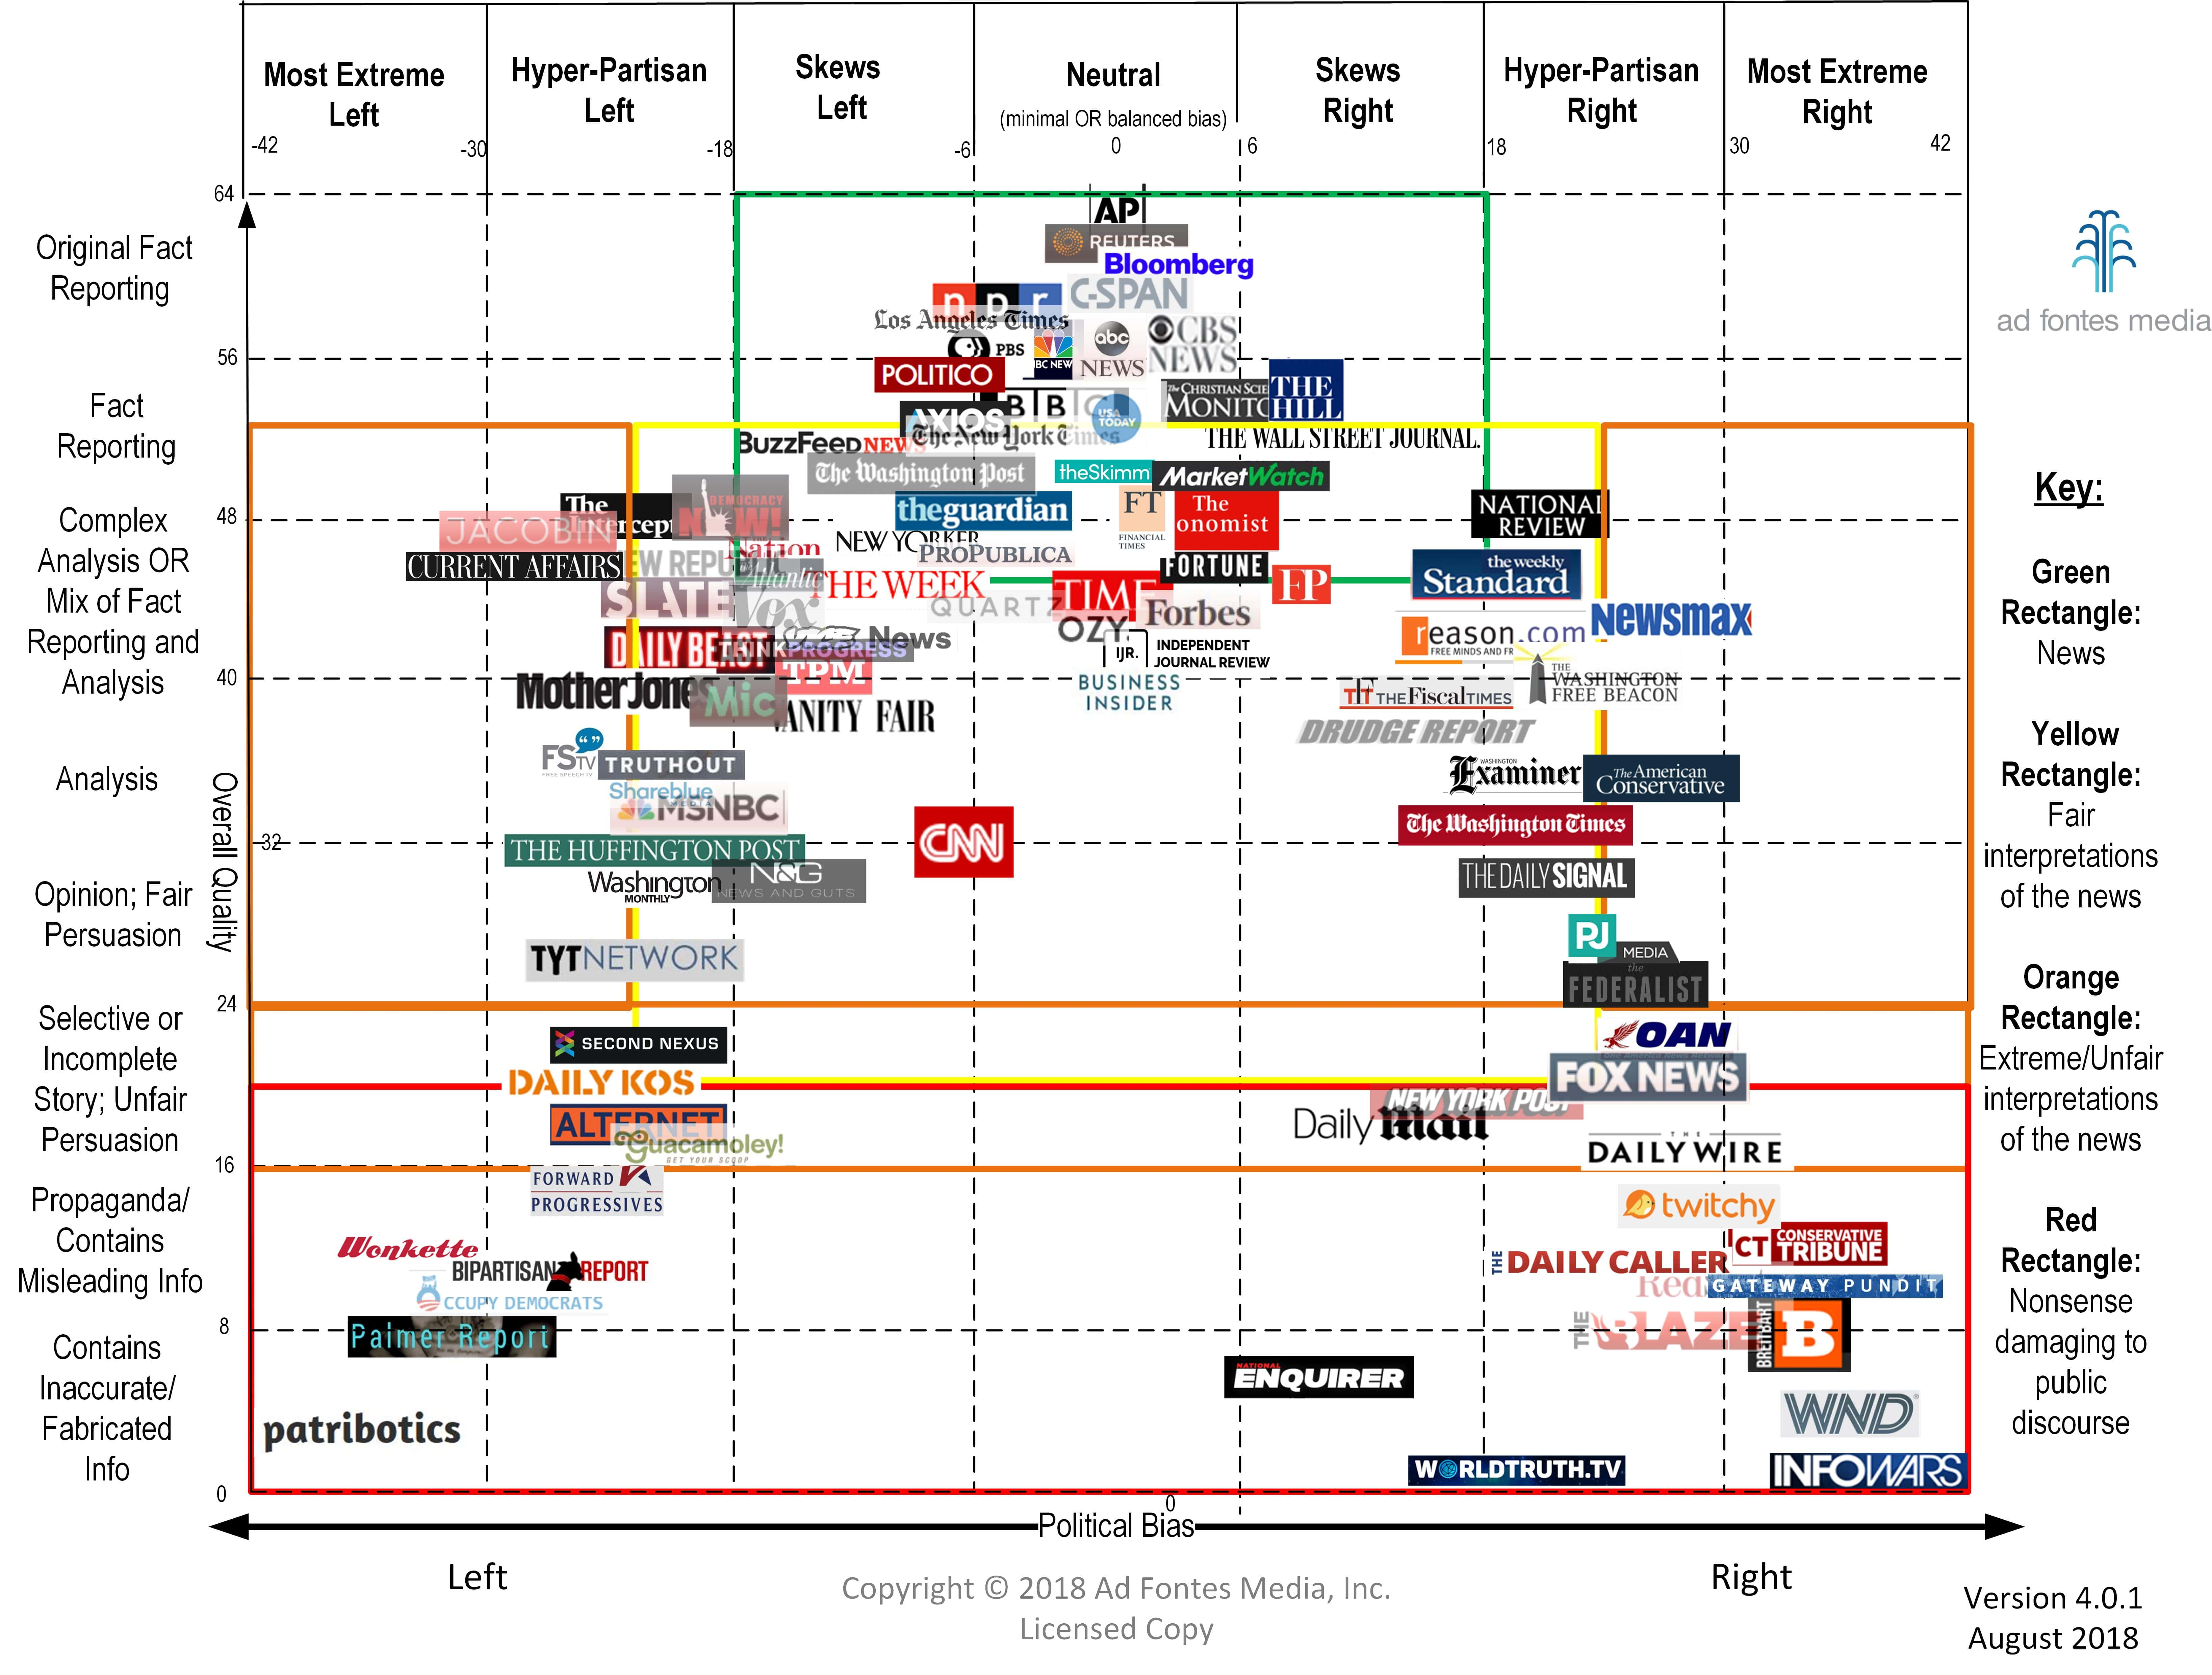
\includegraphics[width=\textwidth]{figures/images/news-bias.jpg}
			\caption{A graphical depiction of the bias in various political news sources.}
			\label{fig:news-bias}
		\end{figure}
	
	%%%%%%%%%%%%%%%%%%%%%%%%%%%%%%%%%%%%%%%%%%%%%%%%
	% DATA
		
	\section{Data}
	    I mined political news articles from the websites of Fox News, Vox News, and PBS News. Importantly, I restricted focus to only URLs that contained an explicit reference to politics i.e. articles from their respective political sections. This allowed me to collect articles that were as similar  as possible to each other in order to try and limit the chances of spurious predictive results. Intuitively, the motivation behind this is to facilitate classification based only on sentiment or semantics, rather than subject matter differences. To better understand how similar the content of these articles are, I construct n-gram tokens and count the frequency of their occurrences. In Table \ref{tab:ngram}, we see the most frequent one, two, and three-gram phrases from the collected corpus.\footnote{The associated counts of each n-gram phrase are shown in Tables \ref{tab:1gram}, \ref{tab:2gram}, and \ref{tab:3gram}, in the Appendix.}
	    
	    \begin{table}[]
    \centering
    \caption{Most frequent words and phrases, by news source.}
    \label{tab:ngram}
    \begin{tabular}{l||l|l|l} 
        
    \hline \hline
    \multicolumn{4}{c}{}                                                                       \\ 
    \multicolumn{4}{c}{\textbf{Most Common Words}}                                             \\ \hline 
        &                             &                            &                             \\
        & \textit{VOX}                & \textit{PBS}               & \textit{FOX}                \\ \hline 
        &                             &                            &                             \\
    1   & trump                       & trump                      & trump                       \\
    2   & tax                         & said                       & said                        \\
    3   & will                        & president                  & president                   \\
    4   & people                      & house                      & house                       \\
    5   & health                      & will                       & new                         \\
    6   & bill                        & new                        & will                        \\
    7   & republicans                 & white                      & democratic                  \\
    8   & one                         & senate                     & democrats                   \\
    9   & new                         & democrats                  & told                        \\
    10  & care                        & campaign                   & border                      \\ \hline \hline % end of first table
    \multicolumn{4}{c}{}                                                                       \\
    \multicolumn{4}{c}{\textbf{Most Common 2-gram Phrases}}                                    \\ \hline
        &                             &                            &                             \\
        & \textit{VOX}                & \textit{PBS}               & \textit{FOX}                \\ \hline 
        &                             &                            &                             \\
    1   & health care                 & white house                & white house                 \\
    2   & white house                 & president donald           & new york                    \\
    3   & trump administration        & donald trump               & president trump             \\
    4   & donald trump                & special counsel            & green new                   \\
    5   & tax cuts                    & supreme court              & health care                 \\
    6   & health insurance            & attorney general           & new deal                    \\
    7   & new york                    & new york                   & united states               \\
    8   & affordable care             & justice department         & border security             \\
    9   & tax bill                    & counsel robert             & donald trump                \\
    10  & federal government          & trump said                 & state union                 \\ \hline \hline % end of second table
    \multicolumn{4}{c}{}                                                                       \\ 
    \multicolumn{4}{c}{\textbf{Most Common 3-gram Phrases}}                                    \\ \hline
        &                             &                            &                             \\
        & \textit{VOX}                & \textit{PBS}               & \textit{FOX}                \\ \hline 
        &                             &                            &                             \\
    1   & affordable care act         & president donald trump     & green new deal              \\ 
    2   & president donald trump      & special counsel robert     & house speaker nancy         \\ 
    3   & congressional budget office & majority leader mitch      & special counsel robert      \\
    4   & health care bill            & attorney general jeff      & partial government shutdown \\
    5   & new york times              & senate judiciary committee & speaker nancy pelosi        \\
    6   & majority leader mitch       & sarah huckabee sanders     & state union address         \\
    7   & american health care        & senate majority leader     & new york times              \\
    8   & leader mitch mcconnell      & counsel robert mueller     & majority leader mitch       \\
    9   & corporate tax rate          & leader mitch mcconnell     & president donald trump      \\
    10  & senate majority leader      & secretary sarah huckabee   & senate majority leader      \\ \hline

    \end{tabular}
\end{table} 
	    
	    Looking carefully at the most common words and phrases we see substantial similarity in terms of topic. Regardless of the source, ``Trump'' is the most used word. Perhaps surprisingly, the top four most used words for PBS and Fox news are exactly the same, and in the same order. Beyond that, we see phrases ``white house'', ``president Donald Trump'', and ``senate majority leader'' appear in the top ten most frequent phrases for each news source. Together, this suggests that, topic wise, the corpus for each source are comparable. 
	    
	    In addition to subject, wording, and phrasing, I also check for grammatical and structural differences with a simple lexical analysis. Using the University of Pennsylvania tagset, I count the percent of adjectives and adverbs in each article and calculate the average for each news source. I find very similar use of adjectives and adverbs for Fox and PBS, and a slightly more frequent use with Vox. Intuitively, the goal is to understand, on average, how descriptive the language is for each source. Toward this end, I included comparatives (e.g. better, worse, greater) and superlatives (e.g. best, worst, greatest) in the count.
	    
	    Finally, I calculate the average number of words per article by source, and the average number of words per sentence, again grouped by news source. Here I find that PBS writes the shortest sentences, while Vox writes the longest. This measure is relevant when considering the average number of words per sentence as a proxy for complexity, as suggested by \citet{flesch1948new}. Table \ref{tab:summary} summarizes these descriptive statistics.  
 
    	\begin{table}[H]
    \centering
    \begin{tabular}{|l|r|r|r|r|r|} \hline
             &                                &                                 &                                       &                                        &                                            \\
             &                                & \multicolumn{1}{c|}{Avg}        &                                       &                                        & \multicolumn{1}{c|}{Avg words}             \\
    Source   & \multicolumn{1}{c|}{Documents} & \multicolumn{1}{c|}{word count} & \multicolumn{1}{c|}{Pct Adjectives}   & \multicolumn{1}{c|}{Pct Adverbs}       & \multicolumn{1}{c|}{per sentence}          \\ \hline \hline
    Fox      & 661                            & 686.2                           & 0.066                                 & 0.034                                  & 20.1                                       \\
    PBS      & 1739                           & 654.3                           & 0.066                                 & 0.032                                  & 18.0                                       \\
    Vox      & 1027                           & 1332.8                          & 0.073                                 & 0.046                                  & 21.3                                       \\ \hline  
    \end{tabular}
    \caption{Summary statistics by data by source. }
    \label{tab:summary}
\end{table}
	    
	\subsection{Challenges} \label{Challenges}
	    There are several limitations to discuss. The most obvious is the difference in corpus size from each source. In particular, Fox News has fewer documents than either PBS or Vox by quite a large number. Fortunately, there are many well established methods for dealing with imbalanced data, like bootstraping, as in \citet{dupret2001bootstrap}. 
	    
	    Second, due to the variability of online formatting, it's worth noting the possibility that, even after cleaning, each source exhibits some subtle idiosyncratic characteristics that could allow a neural network to detect those instead of pure sentiment and semantic differences. To mitigate this, I removed any mention of their own organization, any other common and unique affiliations, and other identifying characteristics.\footnote{For example, I removed any mention of `Fox' from every Fox News article. Similarly, Fox News cited the ``Associated Press'' disproportionately often, so I also removed that string. Additionally, PBS News begins each article with location information in the following format: ``LOCATION --- Start of article...''. In this case, I removed the names of the most frequently referenced cities and the following ``---'' character.} 
	    
	    Finally, each news source shows a difference in the average article length. To overcome this, I limited the article length to a maximum of the first 500 words to ensure that no single source was consistently shorter when fed into the neural network. 
	    
	    \subsection{Statistical Analysis}
	    To get additional context about the contents of the data, I perform a statistical analysis of the data to see what words are most related to the various sources. In particular, \citet{taddy2013multinomial} introduced a framework for using high-dimensional text data in statistical analysis. While I leave the technical details to the paper itself, the intuition is as follows. Suppose we have $N$ documents, each containing some text $x_i$, and a corpus vocabulary that has $p$ distinct tokens. Further, assume that each text document is related to an underlying sentiment $s_i$, whereby the sentiment is influential in creating the text.\footnote{More specifically, imagine that text is generated in accordance with some probability distribution function $g(x_i | s_i)$ as opposed to the sentiment itself being generated, i.e. $f(s_i | x_i)$. The following examples highlight the intuitive differences. One can imagine that saying the phrase ``Country music is fantastic'' is unlikely to \textit{cause} someone to suddenly like country music -- rather, we would suspect that someone who already likes country music would be more likely to say those words. Conversely, if the lead singer of a popular music group said that they will give away backstage passes to the first 10 people to buy tickets to their show, that may cause people to buy tickets, not vice versa.} Since the size of the vocabulary, $p$, can often take values on the order of magnitude 10,000 or more, the simple regression of outcome variable $Y$ on text $X$ (i.e. $Y= \beta X$) will not provide an efficient estimate. What the paper proposed is a method for projecting a document with dimensions $p \times 1$ into a single variable $z_i$ that still preserves information about the sentiment. This technique is useful in part because the first stage multinomial inverse regression allows us to see, pairwise, what phrases are most associated with which source. The following tables below show the results of this first stage multinomial inverse regression. 
	    
	    % latex table generated in R 3.6.0 by xtable 1.8-4 package
% Tue Oct  1 20:21:45 2019
\begin{table}[ht]
\caption{Phrases that are indicitave of either Vox or PBS News.}
\label{tab:vox_pbs}
\centering
\begin{tabular}{rlr|lr}
  \hline
  &             &        &          &        \\
 & \textit{VOX} &  & \textit{PBS} &  \\ 
  \hline
1 & email explain biggest & -6.90 & chairman paul manafort & 6.84 \\ 
  2 & explain biggest news & -6.90 & campaign chairman paul & 6.84 \\ 
  3 & biggest news health & -6.90 & russia trump campaign & 6.84 \\ 
  4 & news health care & -6.90 & mari clare jalonick & 6.83 \\ 
  5 & newslett check newslett & -6.90 & trump campaign chairman & 6.82 \\ 
  6 & check newslett page & -6.90 & mueller russia investig & 6.82 \\ 
  7 & mark email explain & -6.89 & giant timelin everyth & 6.81 \\ 
  8 & health care edit & -6.89 & timelin everyth russia & 6.81 \\ 
  9 & care edit sarah & -6.89 & everyth russia trump & 6.81 \\ 
  10 & edit sarah kliff & -6.89 & russia trump investig & 6.81 \\ 
   \hline
\end{tabular}
\end{table}

	    % latex table generated in R 3.6.0 by xtable 1.8-4 package
% Tue Oct  1 20:22:08 2019
\begin{table}[H]
\caption{Phrases that are indicitave of either PBS or Fox News.}
\label{tab:pbs_fox}
\centering
\begin{tabular}{r||lr|lr}
  \hline \hline
  &             &        &             &        \\
 & \textit{PBS} &  & \textit{FOX} & \\ 
  \hline
1 & washington presid donald & -6.52 & alexandria ocasiocortez dni & 7.36 \\ 
  2 & spoke condit anonym & -6.48 & ongo partial feder & 7.35 \\ 
  3 & mari clare jalonick & -6.45 & york democrat rep & 7.35 \\ 
  4 & timelin everyth russia & -6.44 & alex pappa report & 7.35 \\ 
  5 & everyth russia trump & -6.44 & chad pergram report & 7.34 \\ 
  6 & russia trump investig & -6.44 & presid trump former & 7.34 \\ 
  7 & giant timelin everyth & -6.44 & john robert report & 7.34 \\ 
  8 & read giant timelin & -6.44 & adam shaw report & 7.33 \\ 
  9 & investig russian elect & -6.44 & ap photoj scott & 7.33 \\ 
  10 & author speak publicli & -6.44 & photoj scott applewhit & 7.33 \\ 
   \hline
\end{tabular}
\end{table}

	    % latex table generated in R 3.6.0 by xtable 1.8-4 package
% Tue Oct  1 20:21:23 2019
\begin{table}[H]
\caption{Phrases that are indicitave of either Vox or Fox News.}
\label{tab:vox_fox}
\centering
\begin{tabular}{rlr|lr}
  \hline
  &        &        &         &        \\
 & \textit{VOX} &  & \textit{FOX} &  \\ 
  \hline
  1 & email explain biggest & -6.45 & nanci pelosi dcalif & 7.43 \\ 
  2 & explain biggest news & -6.45 & partial feder govern & 7.43 \\ 
  3 & biggest news health & -6.45 & kamala harri dcalif & 7.43 \\ 
  4 & news health care & -6.45 & elizabeth warren dmass & 7.42 \\ 
  5 & newslett check newslett & -6.45 & ongo partial feder & 7.42 \\ 
  6 & check newslett page & -6.45 & york democrat rep & 7.41 \\ 
  7 & mark email explain & -6.44 & greenhous ga emiss & 7.41 \\ 
  8 & health care edit & -6.44 & major leader steni & 7.40 \\ 
  9 & care edit sarah & -6.44 & leader steni hoyer & 7.40 \\ 
  10 & edit sarah kliff & -6.44 & alex pappa report & 7.40 \\ 
   \hline
\end{tabular}
\end{table}

		
		Here, the magnitude of the number represents how much seeing that phrase contributes to your belief of the underlying news source. So, for example, reading the phrase ``york democrat rep''---which, before stemming refers to the phrase ``[New] York Democrat, representative [...]''---is a good sign that you are reading something written by Fox News. Contextually, the democratic representative from New York is Alexandria Ocasio-Cortez, which also comes up as a signal that the source is Fox News. Interestingly, we notice that seeing the name of a democatratic Congresswomen is a  strong indication that the source is Fox News. Similarly, we see that reading phrases about health care is a sign of a Vox News article. 
		
		Ultimately, this description is valuable insofar as it can help guide our intuition for the particulars of the data, and to help understand some of the similarities and differences between the various sources. 
	
	%%%%%%%%%%%%%%%%%%%%%%%%%%%%%%%%%%%%%%%%%%%%%%%%
	% LSTM MODELS
	    	
	\section{LSTM Models}
	As a baseline, I use long-term short-term memory (LSTM) neural network. The LSTM architecture was introduced in \citet{hochreiter1997long}, and extended the Recurrant Neural Network (RNN) to improve lagged information storage for the purpose of predicting sequential data. The key advantage of the recurrent LSTM architecture is the ability for the cell to ``remember'' relevant lagged values, while ``forgetting'' less useful ones. Visually, we can see a representation of a single LSTM unit in Figure \ref{fig:lstm}.\footnote{Source: https://colah.github.io/posts/2015-08-Understanding-LSTMs}
	
	\begin{figure}[H]
		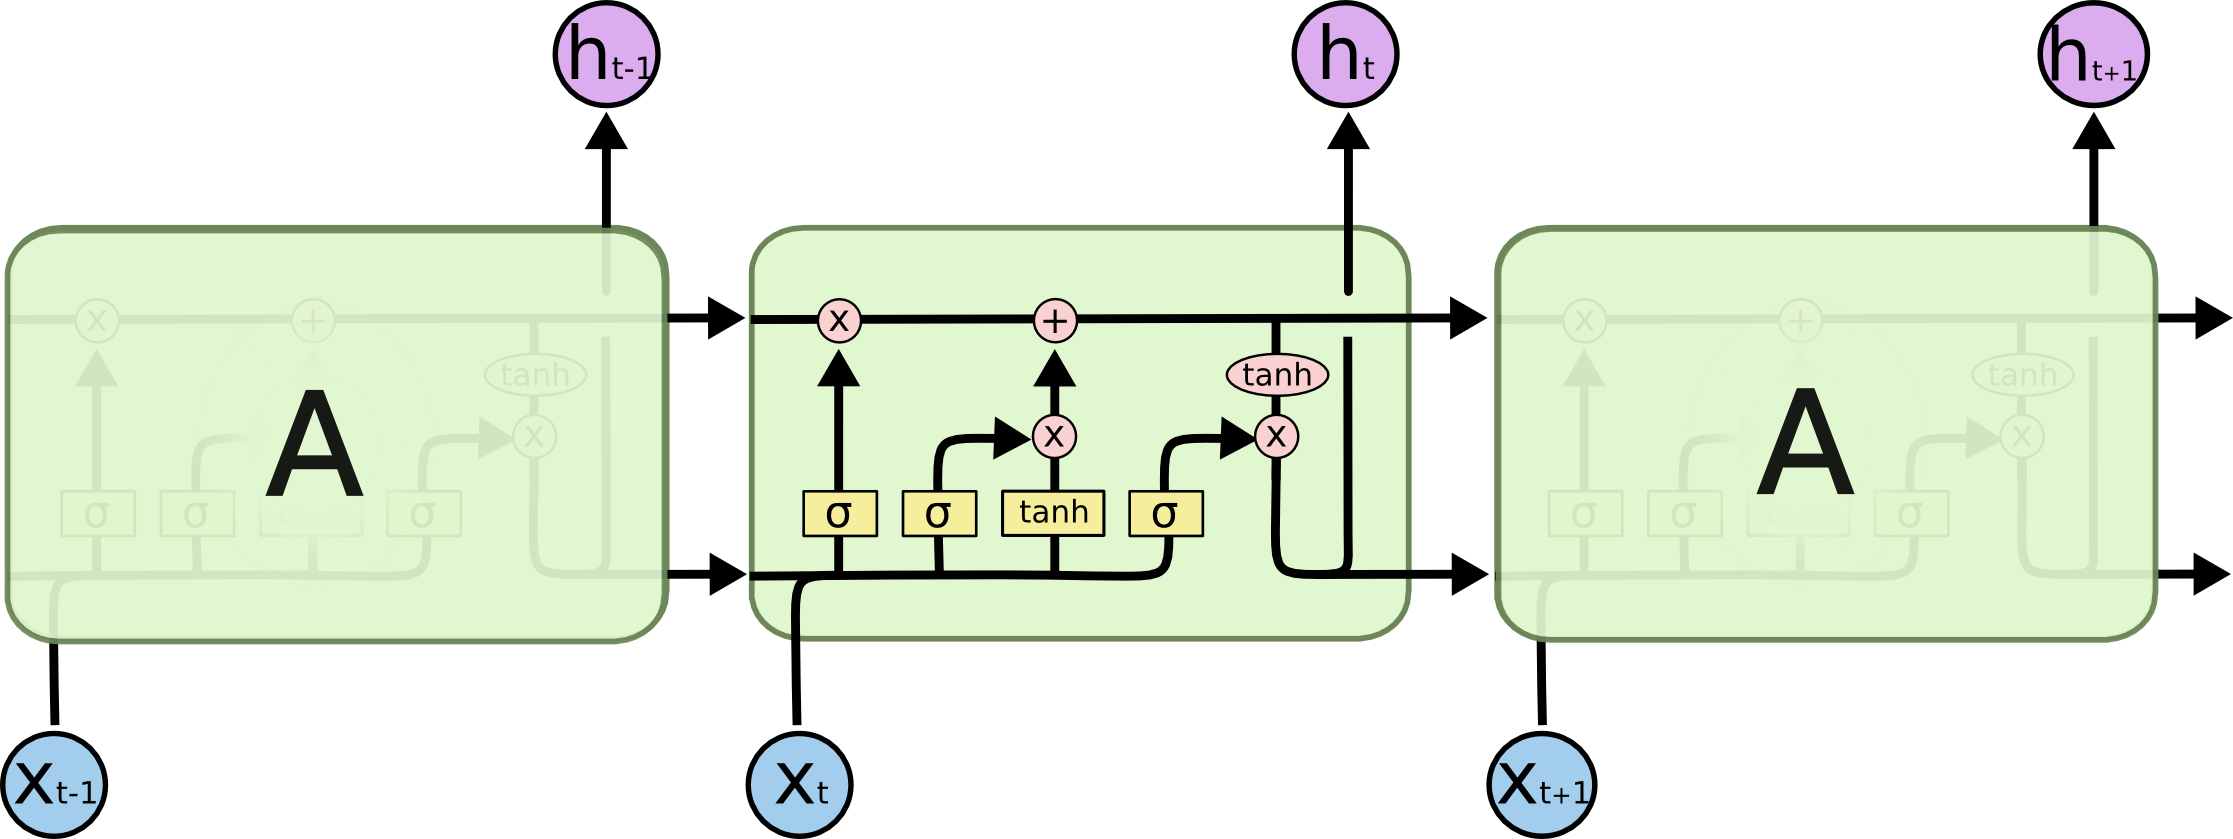
\includegraphics[width=\textwidth]{figures/images/lstm-math.png}
		\caption{A graphical depiction of a single LSTM cell.}
		\label{fig:lstm}
	\end{figure}

	More recently, \citet{gers2000recurrent}, \citet{chung2014empirical}, and \citet{yao2015depth} introduce variations on the baseline \citet{hochreiter1997long} LSTM model, although \citet{greff2016lstm} show them to be roughly equivalent. 
	
	Much success in natural language processing (and other sequential tasks) has been attributed to so-called bidirectional LSTM networks. As in \citet{wang2015unified}, I train an LSTM architecture bidirectionally (i.e. forwards and backwards), and compare it to a unidirectional (i.e. forward-only) baseline. Intuitively, we can think of bidirectional feeds as providing additional context for a given word to ``know'' about what came before it \textit{and} what comes after it. Visually, Figure \ref{fig:bidirectional} depicts a bidirectional network during training. 
	 
	 \begin{figure}[H]
	 	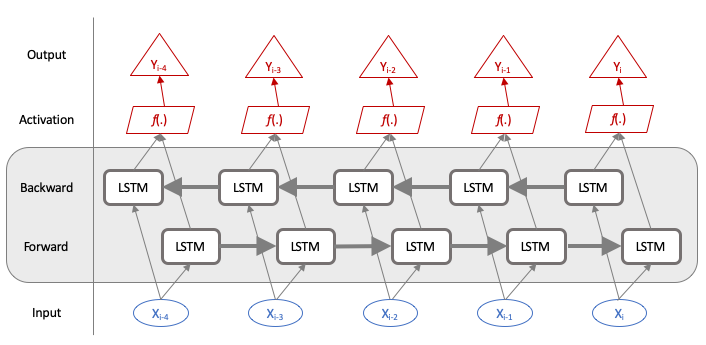
\includegraphics[width=\textwidth]{figures/images/bidirectional-net.png}
	 	\caption{A visual representation of a bidirectional LSTM training.}
	 	\label{fig:bidirectional}
	 \end{figure}
	
	In order to help understand the advantages of training bidirectionally, consider the following sentence. ``The man sat to eat an orange, which, strangely, matched the color of his beard with tremendous accuracy.'' When we as humans read that sentence, we can retroactively modify our understanding. In other words, we can update our image of the man even after he was first mentioned. In this example, when reading the word man, it's possible to first imagine a cleanly shaved man with short dark hair based on the little previous context. However, only \textit{after} finishing the sentence, we can update our mental image to a man with long orange hair and a trimmed beard. Similarly, training the neural network both forward and backward can allow for additional context. 
	
	\subsection{Word Embedding}
	Using the common crawl 840B Global Word Vector (i.e. GloVe), I mapped each word into its corresponding $300 \times 1$ dimensional vector.\footnote{This embedding is introduced in \citet{pennington2014glove} and uses 840 billion tokens and a case-sensitive vocabulary of 2.2 million words to map words into a corresponding $300 \times 1$ dimensional vector.} Since this set of embeddings are case sensitive and unstemmed, I do minimal preprocessing to the text besides the basic cleaning mentioned in Section \ref{Challenges}.
	
	
	%%%%%%%%%%%%%%%%%%%%%%%%%%%%%%%%%%%%%%%%%%%%%%%%
	% RESULTS
		
	\section{Results}
	
	Using bootstrapped data and the setup above, I train and test models with various parameterizations by performing a 90/10 partition of the original dataset into both a training set and testing set for calculating F1 scores. For an RNN, we can specify the batch size, dropout rate, recurrent dropout rate, and the number of steps per epoch. Broadly speaking, batch size describes the number of words included in each training group, the dropout rate specifies the probability of ignoring any given entry in the matrix of weights---this helps to prevent the model from overfitting on any specific word when making predictions. The recurrent dropout, similarly, specifies the dropout that occurs between recurrent cells. Finally, using only one epoch, the steps per epoch represents the number of iterations used in training. 
	
	Results are summarized in Table \ref{tab:bires}. We can see that the results favor a larger batch size, and a larger number of iterations. Perhaps surprisingly, we don't see too much gain from increasing the maximum article length from 250 words to 500 words. This suggests that any linguistic or semantic differences are, in general, noticeable from the start. 
	
	
\begin{table}[H]
    \centering
    \caption{Training results from the bidirectional LSTM, sorted by F1 score.}
    \label{tab:bires}
    \begin{tabular}{c|c|c|c|r|c}
    \hline \hline
    \multicolumn{1}{c}{\textbf{Article}}   & \multicolumn{1}{|c}{\textbf{Batch}}  & \multicolumn{1}{|c}{}                     & \multicolumn{1}{|c}{\textbf{Recurrent}}        & \multicolumn{1}{|c}{\textbf{Steps}}     &  \multicolumn{1}{|c}{}  \\
    \multicolumn{1}{c}{\textbf{Length}}    & \multicolumn{1}{|c}{\textbf{Size}}       & \multicolumn{1}{|c}{\textbf{Dropout}} & \multicolumn{1}{|c}{\textbf{Dropout}}          & \multicolumn{1}{|c}{\textbf{Per Epoch}} & \multicolumn{1}{|c}{\textbf{F1}} \\
    \hline 
    &&&&& \\
    250                                & 64                             & 0.1                         & 0.2                                  & 1000                                & 0.946                  \\
    500                                & 64                             & 0.2                         & 0.2                                  & 1000                                & 0.944                  \\
    500                                & 64                             & 0.2                         & 0.1                                  & 1000                                & 0.939                  \\
    250                                & 64                             & 0.1                         & 0.1                                  & 1000                                & 0.937                  \\
    500                                & 64                             & 0.1                         & 0.1                                  & 1000                                & 0.937                  \\
    500                                & 64                             & 0.1                         & 0.2                                  & 1000                                & 0.933                  \\
    250                                & 64                             & 0.2                         & 0.1                                  & 1000                                & 0.921                  \\
    250                                & 32                             & 0.2                         & 0.1                                  & 1000                                & 0.910                  \\
    250                                & 32                             & 0.1                         & 0.1                                  & 1000                                & 0.906                  \\
    250                                & 64                             & 0.2                         & 0.2                                  & 500                                 & 0.906                  \\
    250                                & 64                             & 0.2                         & 0.2                                  & 1000                                & 0.904                  \\
    500                                & 32                             & 0.1                         & 0.2                                  & 1000                                & 0.904                  \\
    500                                & 32                             & 0.2                         & 0.1                                  & 1000                                & 0.904                  \\
    500                                & 64                             & 0.1                         & 0.1                                  & 500                                 & 0.902                  \\
    500                                & 32                             & 0.1                         & 0.1                                  & 1000                                & 0.900                  \\
    500                                & 64                             & 0.2                         & 0.2                                  & 500                                 & 0.900                  \\
    250                                & 32                             & 0.1                         & 0.2                                  & 1000                                & 0.897                  \\
    250                                & 64                             & 0.1                         & 0.1                                  & 500                                 & 0.897                  \\
    250                                & 64                             & 0.1                         & 0.2                                  & 500                                 & 0.897                  \\
    500                                & 32                             & 0.2                         & 0.2                                  & 1000                                & 0.897                  \\
    250                                & 32                             & 0.2                         & 0.2                                  & 1000                                & 0.895                  \\
    500                                & 64                             & 0.2                         & 0.1                                  & 500                                 & 0.895                  \\
    500                                & 64                             & 0.1                         & 0.2                                  & 500                                 & 0.881                  \\
    250                                & 64                             & 0.2                         & 0.1                                  & 500                                 & 0.877                  \\
    500                                & 32                             & 0.1                         & 0.2                                  & 500                                 & 0.874                  \\
    250                                & 32                             & 0.1                         & 0.1                                  & 500                                 & 0.870                  \\
    250                                & 32                             & 0.2                         & 0.2                                  & 500                                 & 0.860                  \\
    250                                & 32                             & 0.1                         & 0.2                                  & 500                                 & 0.858                  \\
    250                                & 32                             & 0.2                         & 0.1                                  & 500                                 & 0.851                  \\
    500                                & 32                             & 0.2                         & 0.2                                  & 500                                 & 0.845                  \\
    500                                & 32                             & 0.2                         & 0.1                                  & 500                                 & 0.835                  \\
    500                                & 32                             & 0.1                         & 0.1                                  & 500                                 & 0.828                  \\ 
    \hline               
    \end{tabular}
\end{table}

	
	The reported F1 scores are measured across the entire sample by counting the total number of accurate predictions, false positives, and false negatives. Mathematically, the F1 score is the harmonic mean of precision and recall, defined as follows:\footnote{For source, see https://scikit-learn.org/stable/modules/generated/sklearn.metrics.f1\_score.html.} 
	
	\begin{equation*}
		F_1 =  2 \,\, \frac{Precision \cdot Recall}{Precision + Recall}
	\end{equation*}
	
	Where, 
	\begin{align*}
		Precision &= \frac{True Positives}{True Positives + False Positives}\\ \\
		Recall &= \frac{True Positives}{True Positives + False Negatives}
	\end{align*}
	
	As an additional exercise for robustness and comparison, I used similar parameters to train an LSTM recurrent neural network unidirectionally, rather than bidirectionally. Interestingly, we see that the best performing unidirectional model still under performed even the worst performing bidirectional model. Results from this exercise are shown in the Appendix in Figure \ref{tab:unires}.
	
	%%%%%%%%%%%%%%%%%%%%%%%%%%%%%%%%%%%%%%%%%%%%%%%%
	% IMPLEMENTATION
	
	\section{Implementation}
	
	To make use of this trained model in application, I wrote a simple web interface that enables passing text from an arbitrary news article through a form, and returns values that can be interpreted as predictions of the likelihood that a given article is from Fox, Vox, or PBS News. The commercial use case for this type of app is to provide context as to the type of writing, either before or after the consumer has read the article. Ideally, each user could login and see a history of the news they consume---this could help interested readers identify if and when they are in a political bubble or echo-chamber. Idealistically, it could help balance information consumption. 
	
	Extensions of this work would include more volume and more recent news articles as to stay current with changing topics and trends. Additional news sources would also be desirable for readers to chose their set of comparisons such that they are comfortable in assessing the relative balance and neutrality of the set as a whole. 
	
	A sample of the interface is shown in Figures \ref{fig:form} and \ref{fig:results} below. 	
	
	\begin{figure}[H]
		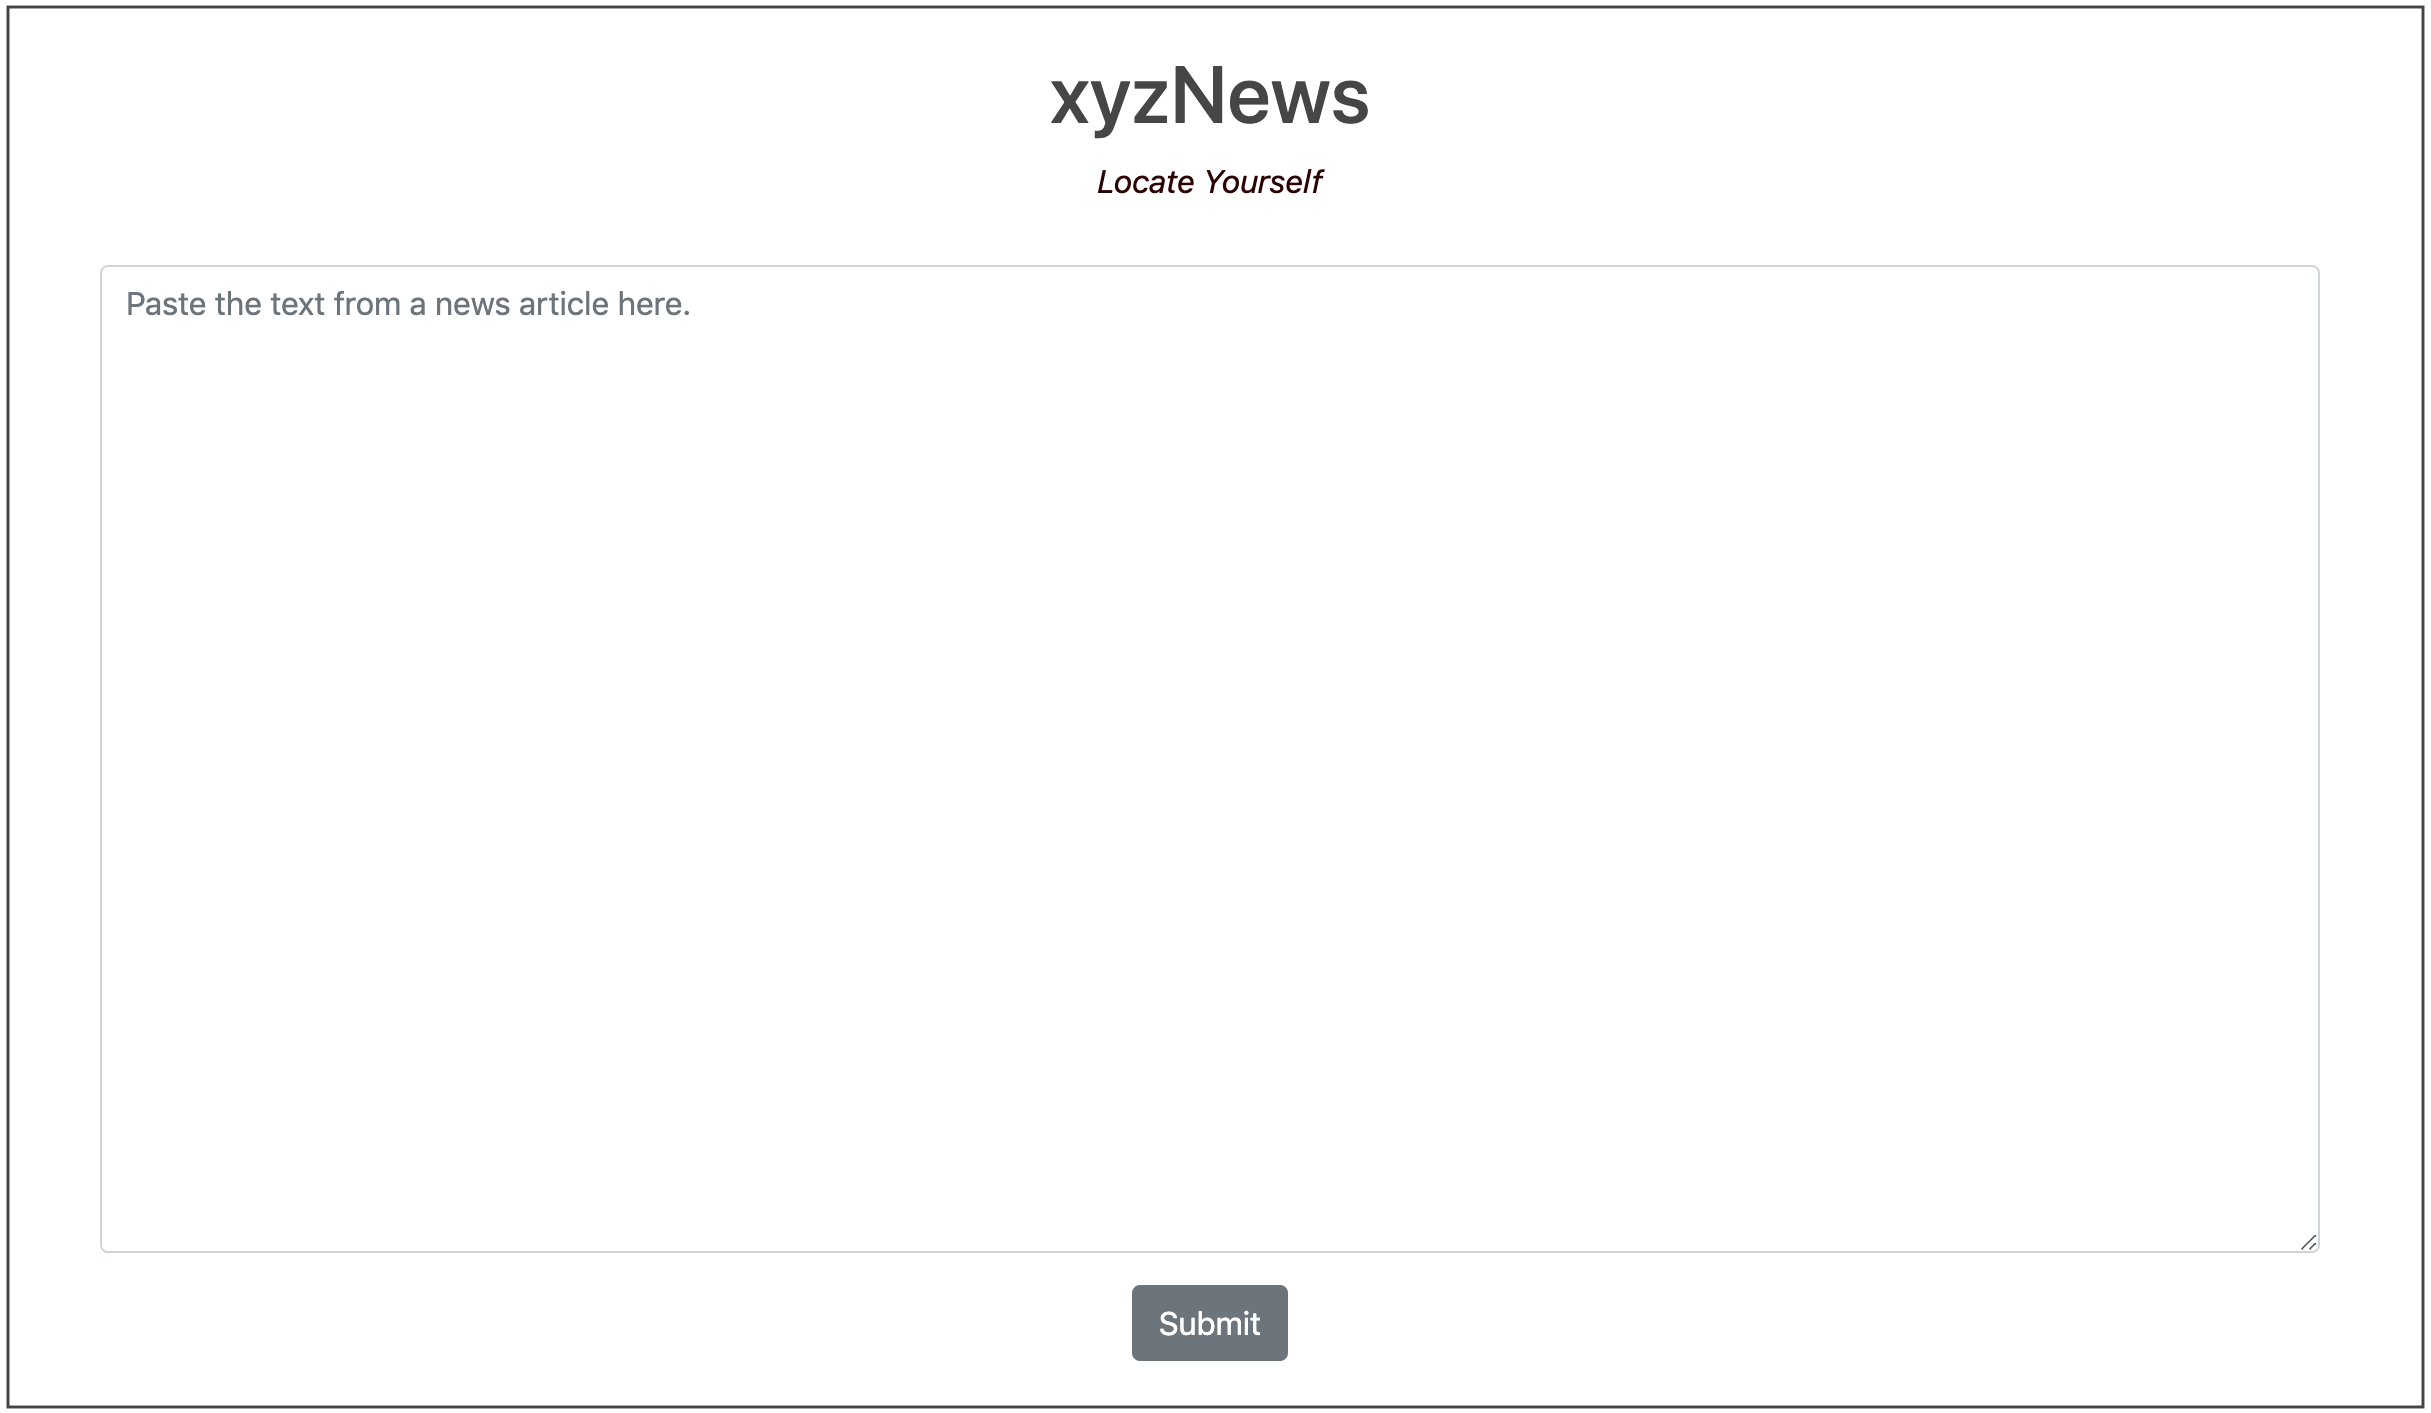
\includegraphics[width=\textwidth]{figures/images/web-form.png}
		\caption{The web app's home page.}
		\label{fig:form}
	\end{figure}

	\begin{figure}[H]
		\centering
		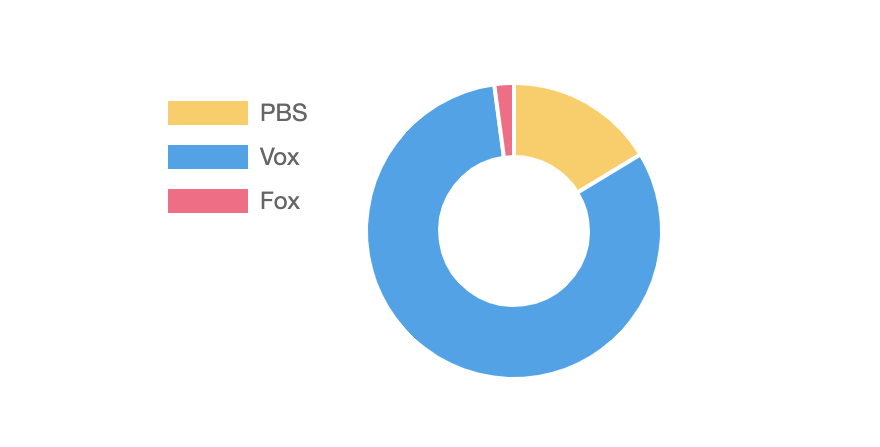
\includegraphics[width=0.75\textwidth]{figures/images/web-results.png}
		\caption{The display of prediction results.}
		\label{fig:results}
	\end{figure}

	%%%%%%%%%%%%%%%%%%%%%%%%%%%%%%%%%%%%%%%%%%%%%%%%
	% CONCLUSION
		
	\section{Conclusion and Discussion}
	I've shown that a neural network can accurately classify news articles based on language differences in the underlying news sources. These results have implications for our politically polarized world, where even scientific ``facts'' are now often disputed. While there are plenty of factors that could motivate news companies to intentionally bias their news,  \citet{gentzkow2008competition} and \citet{gentzkow2006media} suggest that the profit maximizing response of a company is to produce a news product that confirms consumers prior beliefs. Thus, given a society of individuals with heterogeneous preferences and beliefs, and a competitive news information market, it seems unlikely that biased news (or even fake news) will disappear anytime soon. 
	
	A software application based on the ideas presented above could serve as a starting point to measure news consumption---much in the same way that calendars can help to measure our time use, nutrition apps measure our consumption of macronutrients, and GPS measures our geographical position. 
	
	\newpage
	
	%%%%%%%%%%%%%%%%%%%%%%%%%%%%%%%%%%%%%%%%%%%%%%%%
	% REFERENCES
	
	\bibliographystyle{plainnat}
	\bibliography{references/ref}
	
	\newpage
	
	%%%%%%%%%%%%%%%%%%%%%%%%%%%%%%%%%%%%%%%%%%%%%%%%
	% APPENDIX
	
	\section{Appendix}
	
	\begin{center}
		\begin{table}[H]
    \centering
    \caption{Word Frequencies}
    \label{tab:1gram}
    \begin{tabular}{l|l|l|l} \hline
    \textbf{Num} & \textbf{Vox} & \textbf{PBS} & \textbf{Fox} \\ \hline \hline
    &&& \\
    1   & trump       & trump     & trump      \\
    2   & tax         & said      & said       \\
    3   & will        & president & president  \\
    4   & people      & house     & house      \\
    5   & health      & will      & new        \\
    6   & bill        & new       & will       \\
    7   & republicans & white     & democratic \\
    8   & one         & senate    & democrats  \\
    9   & new         & democrats & told       \\
    10  & care        & campaign  & border     \\ \hline
    \end{tabular}
\end{table}
		
		\begin{table}[H]
    \centering
    \caption{Top frequencies of two word phrases.}
    \label{tab:2gram}
    \begin{tabular}{l|lr|lr|lr}
    \hline
    \textbf{Num} & \multicolumn{2}{c|}{\textbf{Vox}}           & \multicolumn{2}{c|}{\textbf{PBS}}          & \multicolumn{2}{c}{\textbf{Fox}} \\ \hline \hline
    &&&&&& \\
    1   & health care          & 1654 & white house        & 1683 & white house     & 556 \\
    2   & white house          & 743  & president donald   & 1297 & new york        & 359 \\
    3   & trump administration & 672  & donald trump       & 1035 & president trump & 318 \\
    4   & donald trump         & 598  & special counsel    & 613  & green new       & 256 \\
    5   & tax cuts             & 479  & supreme court      & 584  & health care     & 160 \\
    6   & health insurance     & 479  & attorney general   & 499  & new deal        & 151 \\
    7   & new york             & 470  & new york           & 491  & united states   & 134 \\
    8   & affordable care      & 437  & justice department & 485  & border security & 132 \\
    9   & tax bill             & 376  & counsel robert     & 405  & donald trump    & 131 \\
    10  & federal government   & 365  & trump said         & 369  & state union     & 126 \\ \hline
    \end{tabular}
\end{table}
		
		
\begin{table}[H]
    \caption{Top frequencies of three word phrases.}
    \label{tab:3gram}
    \begin{tabular}{l|ll|ll|ll}
    \hline
    Num & \multicolumn{2}{c|}{Vox}          & \multicolumn{2}{c|}{PBS}         & \multicolumn{2}{c}{Fox}          \\ \hline \hline
    1   & affordable care act         & 222 & president donald trump     & 785 & green new deal              & 143 \\ 
    2   & president donald trump      & 157 & special counsel robert     & 396 & house speaker nancy         & 81  \\ 
    3   & congressional budget office & 127 & majority leader mitch      & 179 & special counsel robert      & 72  \\
    4   & health care bill            & 121 & attorney general jeff      & 139 & partial government shutdown & 63  \\
    5   & new york times              & 115 & senate judiciary committee & 137 & speaker nancy pelosi        & 58  \\
    6   & majority leader mitch       & 114 & sarah huckabee sanders     & 137 & state union address         & 53  \\
    7   & american health care        & 97  & senate majority leader     & 131 & new york times              & 51  \\
    8   & leader mitch mcconnell      & 96  & counsel robert mueller     & 123 & majority leader mitch       & 47  \\
    9   & corporate tax rate          & 95  & leader mitch mcconnell     & 113 & president donald trump      & 43  \\
    10  & senate majority leader      & 95  & secretary sarah huckabee   & 108 & senate majority leader      & 41  \\ \hline
    \end{tabular}
\end{table}

		
		\begin{table}[H]
    \centering
    \caption{Training results from the unidirectional LSTM, sorted by F1 score.}
    \label{tab:unires}
    \begin{tabular}{c|c|c|c|r|c}
    \multicolumn{1}{c}{\textbf{Article}}   & \multicolumn{1}{|c}{\textbf{Batch}}  & \multicolumn{1}{|c}{}                     & \multicolumn{1}{|c}{\textbf{Recurrent}}        & \multicolumn{1}{|c}{\textbf{Steps}}     &  \multicolumn{1}{|c}{}  \\
    \multicolumn{1}{c}{\textbf{Length}}    & \multicolumn{1}{|c}{\textbf{Size}}       & \multicolumn{1}{|c}{\textbf{Dropout}} & \multicolumn{1}{|c}{\textbf{Dropout}}          & \multicolumn{1}{|c}{\textbf{Per Epoch}} & \multicolumn{1}{|c}{\textbf{F1}} \\
    \hline 
    &&&&& \\
    250                                & 64                             & 0.2                         & 0.1                                  & 1000                                & 0.824                  \\
    250                                & 64                             & 0.1                         & 0.2                                  & 1000                                & 0.797                  \\
    250                                & 32                             & 0.1                         & 0.2                                  & 1000                                & 0.766                  \\
    500                                & 64                             & 0.1                         & 0.1                                  & 1000                                & 0.724                  \\
    250                                & 64                             & 0.2                         & 0.2                                  & 1000                                & 0.716                  \\
    250                                & 32                             & 0.2                         & 0.1                                  & 1000                                & 0.703                  \\
    500                                & 64                             & 0.2                         & 0.2                                  & 1000                                & 0.703                  \\
    250                                & 32                             & 0.2                         & 0.2                                  & 1000                                & 0.695                  \\
    250                                & 64                             & 0.1                         & 0.2                                  & 500                                 & 0.686                  \\
    250                                & 64                             & 0.2                         & 0.2                                  & 500                                 & 0.686                  \\
    500                                & 64                             & 0.2                         & 0.1                                  & 1000                                & 0.678                  \\
    250                                & 64                             & 0.2                         & 0.1                                  & 500                                 & 0.670                  \\
    250                                & 32                             & 0.1                         & 0.1                                  & 1000                                & 0.653                  \\
    250                                & 64                             & 0.1                         & 0.1                                  & 500                                 & 0.653                  \\
    250                                & 64                             & 0.1                         & 0.1                                  & 1000                                & 0.653                  \\
    500                                & 32                             & 0.1                         & 0.2                                  & 1000                                & 0.644                  \\
    250                                & 32                             & 0.2                         & 0.1                                  & 500                                 & 0.640                  \\
    250                                & 32                             & 0.2                         & 0.2                                  & 500                                 & 0.628                  \\
    250                                & 32                             & 0.1                         & 0.2                                  & 500                                 & 0.619                  \\
    250                                & 32                             & 0.1                         & 0.1                                  & 500                                 & 0.607                  \\
    500                                & 64                             & 0.1                         & 0.2                                  & 500                                 & 0.607                  \\
    500                                & 64                             & 0.1                         & 0.2                                  & 1000                                & 0.602                  \\
    500                                & 32                             & 0.2                         & 0.1                                  & 1000                                & 0.600                  \\
    500                                & 64                             & 0.2                         & 0.2                                  & 500                                 & 0.598                  \\
    500                                & 32                             & 0.2                         & 0.2                                  & 500                                 & 0.594                  \\
    500                                & 32                             & 0.1                         & 0.2                                  & 500                                 & 0.592                  \\
    500                                & 32                             & 0.1                         & 0.1                                  & 1000                                & 0.584                  \\
    500                                & 32                             & 0.1                         & 0.1                                  & 500                                 & 0.579                  \\
    500                                & 32                             & 0.2                         & 0.2                                  & 1000                                & 0.571                  \\
    500                                & 64                             & 0.1                         & 0.1                                  & 500                                 & 0.565                  \\
    500                                & 32                             & 0.2                         & 0.1                                  & 500                                 & 0.559                  \\
    500                                & 64                             & 0.2                         & 0.1                                  & 500                                 & 0.556                  \\
    \hline               
\end{tabular}
\end{table}
	\end{center}
	
\end{document}